% figures/specialization-key-cache.tex
% Specialization key composition and the verify-or-reject persistent
% cache path.
\documentclass[tikz,border=10pt]{standalone}
% figures/common-preamble.tex
% Shared setup for the TikZ documentation figures. Colors mirror the
% palette in scripts/render_docs_diagrams.py so both atlases match.
\usepackage[T1]{fontenc}
\usepackage{lmodern}
\usepackage{tikz}
\usepackage{pgfplots}
\pgfplotsset{compat=1.18}
\usetikzlibrary{arrows.meta}
\usetikzlibrary{backgrounds}
\usetikzlibrary{calc}
\usetikzlibrary{decorations.pathreplacing}
\usetikzlibrary{fit}
\usetikzlibrary{positioning}

\definecolor{swcanvas}{HTML}{FFFDF8}
\definecolor{swpanel}{HTML}{F5F3ED}
\definecolor{swink}{HTML}{17212B}
\definecolor{swmuted}{HTML}{4B5563}
\definecolor{swline}{HTML}{59636E}
\definecolor{swblue}{HTML}{00689D}
\definecolor{swbluefill}{HTML}{DCEFFD}
\definecolor{swpurple}{HTML}{8E4775}
\definecolor{swpurplefill}{HTML}{F7E2EF}
\definecolor{sworange}{HTML}{A94500}
\definecolor{sworangefill}{HTML}{FCE5DC}
\definecolor{swgreen}{HTML}{00664B}
\definecolor{swgreenfill}{HTML}{DDF4EB}
\definecolor{swgrayfill}{HTML}{EEF0F2}

\pagecolor{swcanvas}
\AtBeginDocument{\color{swink}}

\tikzset{
  swcell/.style={
    draw, minimum width=0.46cm, minimum height=0.46cm, inner sep=0pt,
    line width=0.7pt, rounded corners=1pt},
  swbox/.style={
    draw=swline, fill=swpanel, rounded corners=6pt, line width=0.9pt},
  swarrow/.style={-{Stealth[length=6pt]}, draw=swline, line width=1pt},
  swtag/.style={
    draw, rounded corners=8pt, line width=0.9pt,
    font=\bfseries\scriptsize, inner xsep=8pt, inner ysep=4pt},
  swtitle/.style={anchor=west, font=\Large\bfseries, text=swink},
  swsubtitle/.style={anchor=west, font=\small, text=swmuted},
  swcode/.style={font=\small\ttfamily, text=swink},
  every picture/.style={line cap=round},
}

\begin{document}
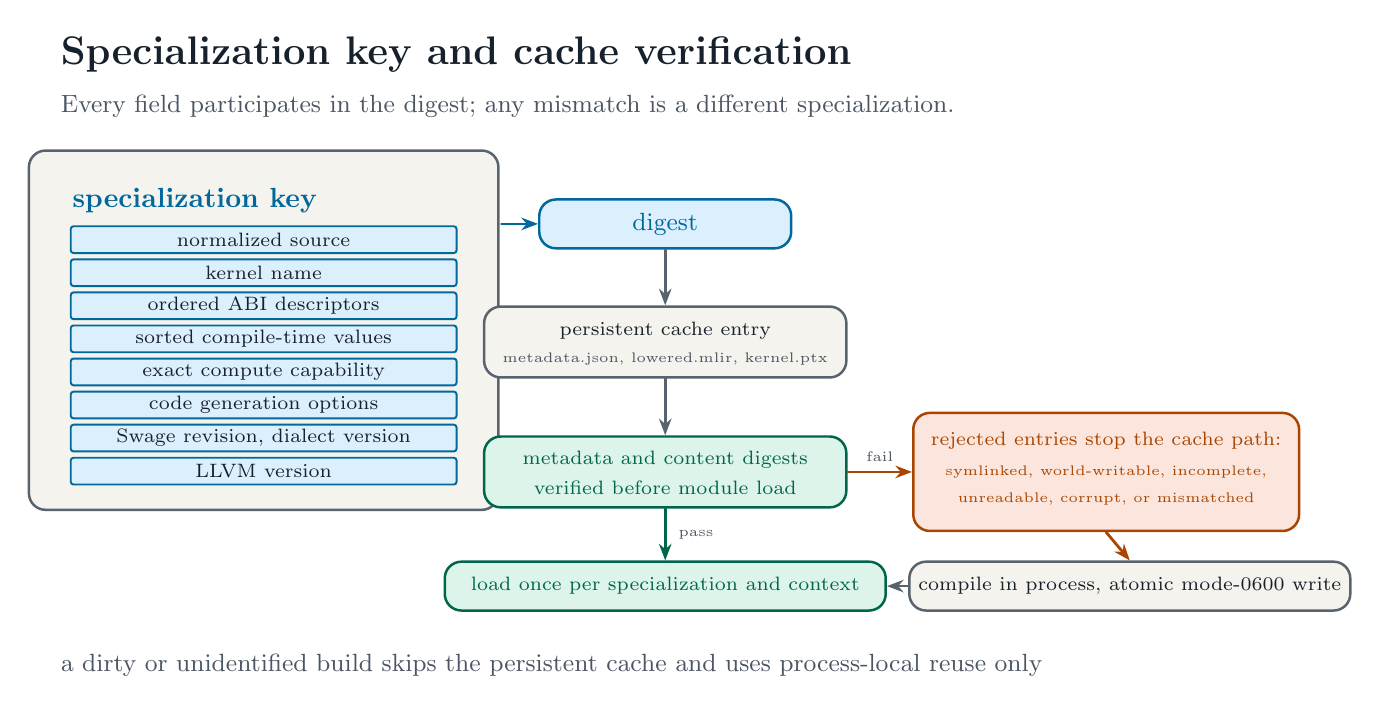
\begin{tikzpicture}[x=1cm, y=1cm]

% Header.
\node[swtitle] at (0, 1.15) {Specialization key and cache verification};
\node[swsubtitle] at (0, 0.5)
  {Every field participates in the digest; any mismatch is a
   different specialization.};

% The specialization key fields.
\node[swbox, fit={(0, -4.35) (5.4, -0.35)}, inner sep=8pt] {};
\node[anchor=west, font=\bfseries, text=swblue] at (0.15, -0.7)
  {specialization key};
\foreach \row/\field in {%
    0/{normalized source},
    1/{kernel name},
    2/{ordered ABI descriptors},
    3/{sorted compile-time values},
    4/{exact compute capability},
    5/{code generation options},
    6/{Swage revision, dialect version},
    7/{LLVM version}} {
  \node[swcell, minimum width=4.9cm, minimum height=0.34cm,
        fill=swbluefill, draw=swblue]
    at (2.7, {-1.2 - \row * 0.42}) {};
  \node[font=\scriptsize, text=swink]
    at (2.7, {-1.2 - \row * 0.42}) {\field};
}

% Digest and lookup flow.
\node[swbox, draw=swblue, fill=swbluefill, minimum width=3.2cm,
      minimum height=0.62cm] (digest) at (7.8, -1.0) {};
\node[font=\small, text=swblue] at (7.8, -1.0) {digest};
\draw[swarrow, draw=swblue] (5.72, -1.0) -- (digest.west);

\node[swbox, minimum width=4.6cm, minimum height=0.9cm]
  (lookup) at (7.8, -2.5) {};
\node[font=\scriptsize, text=swink, align=center] at (7.8, -2.35)
  {persistent cache entry};
\node[font=\tiny, text=swmuted, align=center] at (7.8, -2.72)
  {metadata.json, lowered.mlir, kernel.ptx};
\draw[swarrow] (digest.south) -- (lookup.north);

\node[swbox, draw=swgreen, fill=swgreenfill, minimum width=4.6cm,
      minimum height=0.9cm] (verify) at (7.8, -4.15) {};
\node[font=\scriptsize, text=swgreen, align=center] at (7.8, -4.0)
  {metadata and content digests};
\node[font=\scriptsize, text=swgreen, align=center] at (7.8, -4.35)
  {verified before module load};
\draw[swarrow] (lookup.south) -- (verify.north);

\node[swbox, draw=swgreen, fill=swgreenfill, minimum width=5.6cm,
      minimum height=0.62cm] (load) at (7.8, -5.6) {};
\node[font=\scriptsize, text=swgreen] at (7.8, -5.6)
  {load once per specialization and context};
\draw[swarrow, draw=swgreen] (verify.south) -- (load.north)
  node[midway, right=1pt, font=\tiny, text=swmuted] {pass};

% Rejection and recompilation.
\node[swbox, draw=sworange, fill=sworangefill, minimum width=4.9cm,
      minimum height=1.5cm] (reject) at (13.4, -4.15) {};
\node[font=\scriptsize, text=sworange, align=center] at (13.4, -3.75)
  {rejected entries stop the cache path:};
\node[font=\tiny, text=sworange, align=center] at (13.4, -4.15)
  {symlinked, world-writable, incomplete,};
\node[font=\tiny, text=sworange, align=center] at (13.4, -4.5)
  {unreadable, corrupt, or mismatched};
\draw[swarrow, draw=sworange] (verify.east) -- (reject.west)
  node[midway, above=0pt, font=\tiny, text=swmuted] {fail};

\node[swbox, minimum width=5.6cm, minimum height=0.62cm]
  (compile) at (13.7, -5.6) {};
\node[font=\scriptsize, text=swink] at (13.7, -5.6)
  {compile in process, atomic mode-0600 write};
\draw[swarrow, draw=sworange] (reject.south) -- (compile.north);
\draw[swarrow] (compile.west) -- (load.east);

% Scope note.
\node[anchor=west, font=\small, text=swmuted] at (0, -6.6)
  {a dirty or unidentified build skips the persistent cache and uses
   process-local reuse only};

\end{tikzpicture}
\end{document}
